\chapter{Background}

\section{Distributed Ledger Technology}

\section{Manufacture Usage Description}

MUD has been developed by the International Engineering Task Force, IETF, with following goals and intents in mind:
\cite{rfc8520-mud}
\begin{itemize}
	\item Substantially reduce the threat surface on a device to those communications intended by the manufacturer.
	\item Provide a means to scale network policies to the ever-increasing number of types of devices in the network.
	\item Provide a means to address at least some vulnerabilities in a way that is faster than the time it might
	      take to update systems. This will be particularly true for systems that are no longer supported.
	\item Keep the cost of implementation of such a system to the bare minimum.
	\item Provide a means of extensibility for manufacturers to express other device capabilities or requirements.
\end{itemize}

MUD does not entail address network authorization of general purpose computers, it simply creates a suggestion than can
be followed.
The architecture of Devices using MUD can be seen in Figure~\ref{fig:NIST MUD Reference Architecture}, which is the
reference architecture by NIST \cite{dodson2021securing} but it can be found in similar fashion inside the RFC
specification.

\begin{figure}
	\begin{center}
		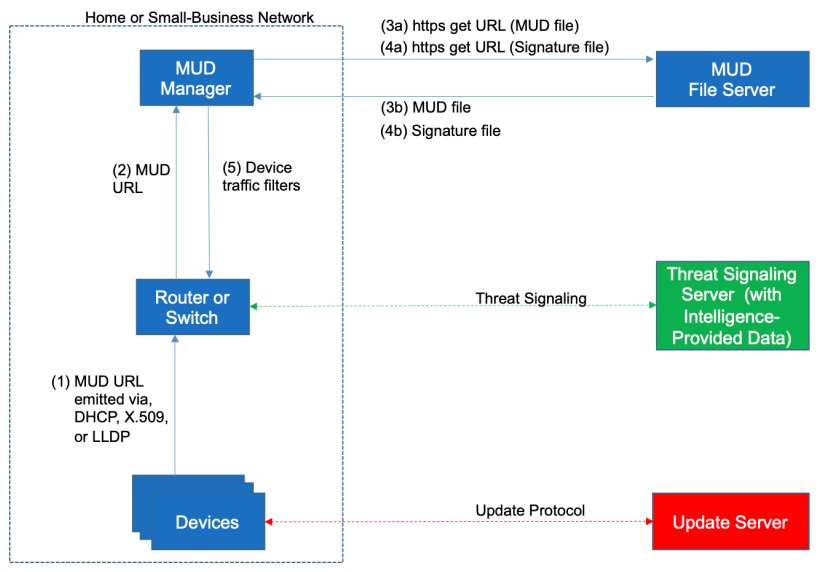
\includegraphics[width=0.95\textwidth]{figures/nist-mud-arch.png}
	\end{center}
	\caption{NIST MUD Reference Architecture}
	\label{fig:NIST MUD Reference Architecture}
\end{figure}
